\documentclass[tikz,border=5pt]{standalone}
\usepackage{amsmath,amssymb}
\usepackage{fontspec}
\setmainfont{Arial}
\setsansfont{Arial}
\renewcommand{\familydefault}{\sfdefault}
\usepackage{xcolor}
\usepackage{tikz}
\usetikzlibrary{arrows.meta,calc,fit,positioning}

\definecolor{greenfill}{HTML}{DCEBD2}
\definecolor{greendraw}{HTML}{64845B}
\definecolor{redfill}{HTML}{E7B6AD}
\definecolor{reddraw}{HTML}{A75A50}
\definecolor{bluefill}{HTML}{C8DDF0}
\definecolor{bluedraw}{HTML}{557A9A}
\definecolor{navyfill}{HTML}{D5E1ED}
\definecolor{navydraw}{HTML}{3F607D}
\definecolor{yellowfill}{HTML}{FFF0C8}
\definecolor{yellowdraw}{HTML}{A48743}
\definecolor{grayfill}{HTML}{EEEEEE}
\definecolor{graydraw}{HTML}{666666}
\definecolor{purplefill}{HTML}{E5D4E2}
\definecolor{purpledraw}{HTML}{8D6788}
\definecolor{ink}{HTML}{171717}

\tikzset{
  >=Latex,
  flow/.style={draw=ink, line width=0.75pt, -{Latex[length=2.2mm,width=1.5mm]}},
  feedback/.style={draw=ink, line width=0.70pt, -{Latex[length=2.1mm,width=1.45mm]}},
  informative/.style={draw=ink!75, dashed, line width=0.70pt, -{Latex[length=2.1mm,width=1.45mm]}},
  block/.style={
    rounded corners=2.0mm,
    draw=graydraw,
    fill=grayfill,
    line width=0.8pt,
    align=center,
    font=\bfseries\small,
    inner sep=3.0mm
  },
  analytic/.style={block, fill=grayfill, draw=graydraw},
  fixed/.style={block, fill=greenfill, draw=greendraw},
  learned/.style={block, fill=redfill, draw=reddraw},
  gate/.style={block, fill=bluefill, draw=bluedraw},
  control/.style={block, fill=yellowfill, draw=yellowdraw},
  perception/.style={block, fill=purplefill, draw=purpledraw},
  subblock/.style={
    rounded corners=1.2mm,
    draw=navydraw,
    fill=navyfill,
    line width=0.6pt,
    align=center,
    font=\bfseries\scriptsize,
    inner sep=1.8mm
  },
  smalllabel/.style={font=\itshape\scriptsize, align=center, text=ink},
  stage/.style={font=\bfseries\large, anchor=west, text=ink},
  panel/.style={font=\bfseries\Large, fill=grayfill, inner xsep=6mm, inner ysep=1mm},
  tag/.style={
    rounded corners=0.8mm,
    draw=graydraw,
    fill=white,
    line width=0.45pt,
    font=\bfseries\tiny,
    inner xsep=1.3mm,
    inner ysep=0.6mm
  }
}

\begin{document}
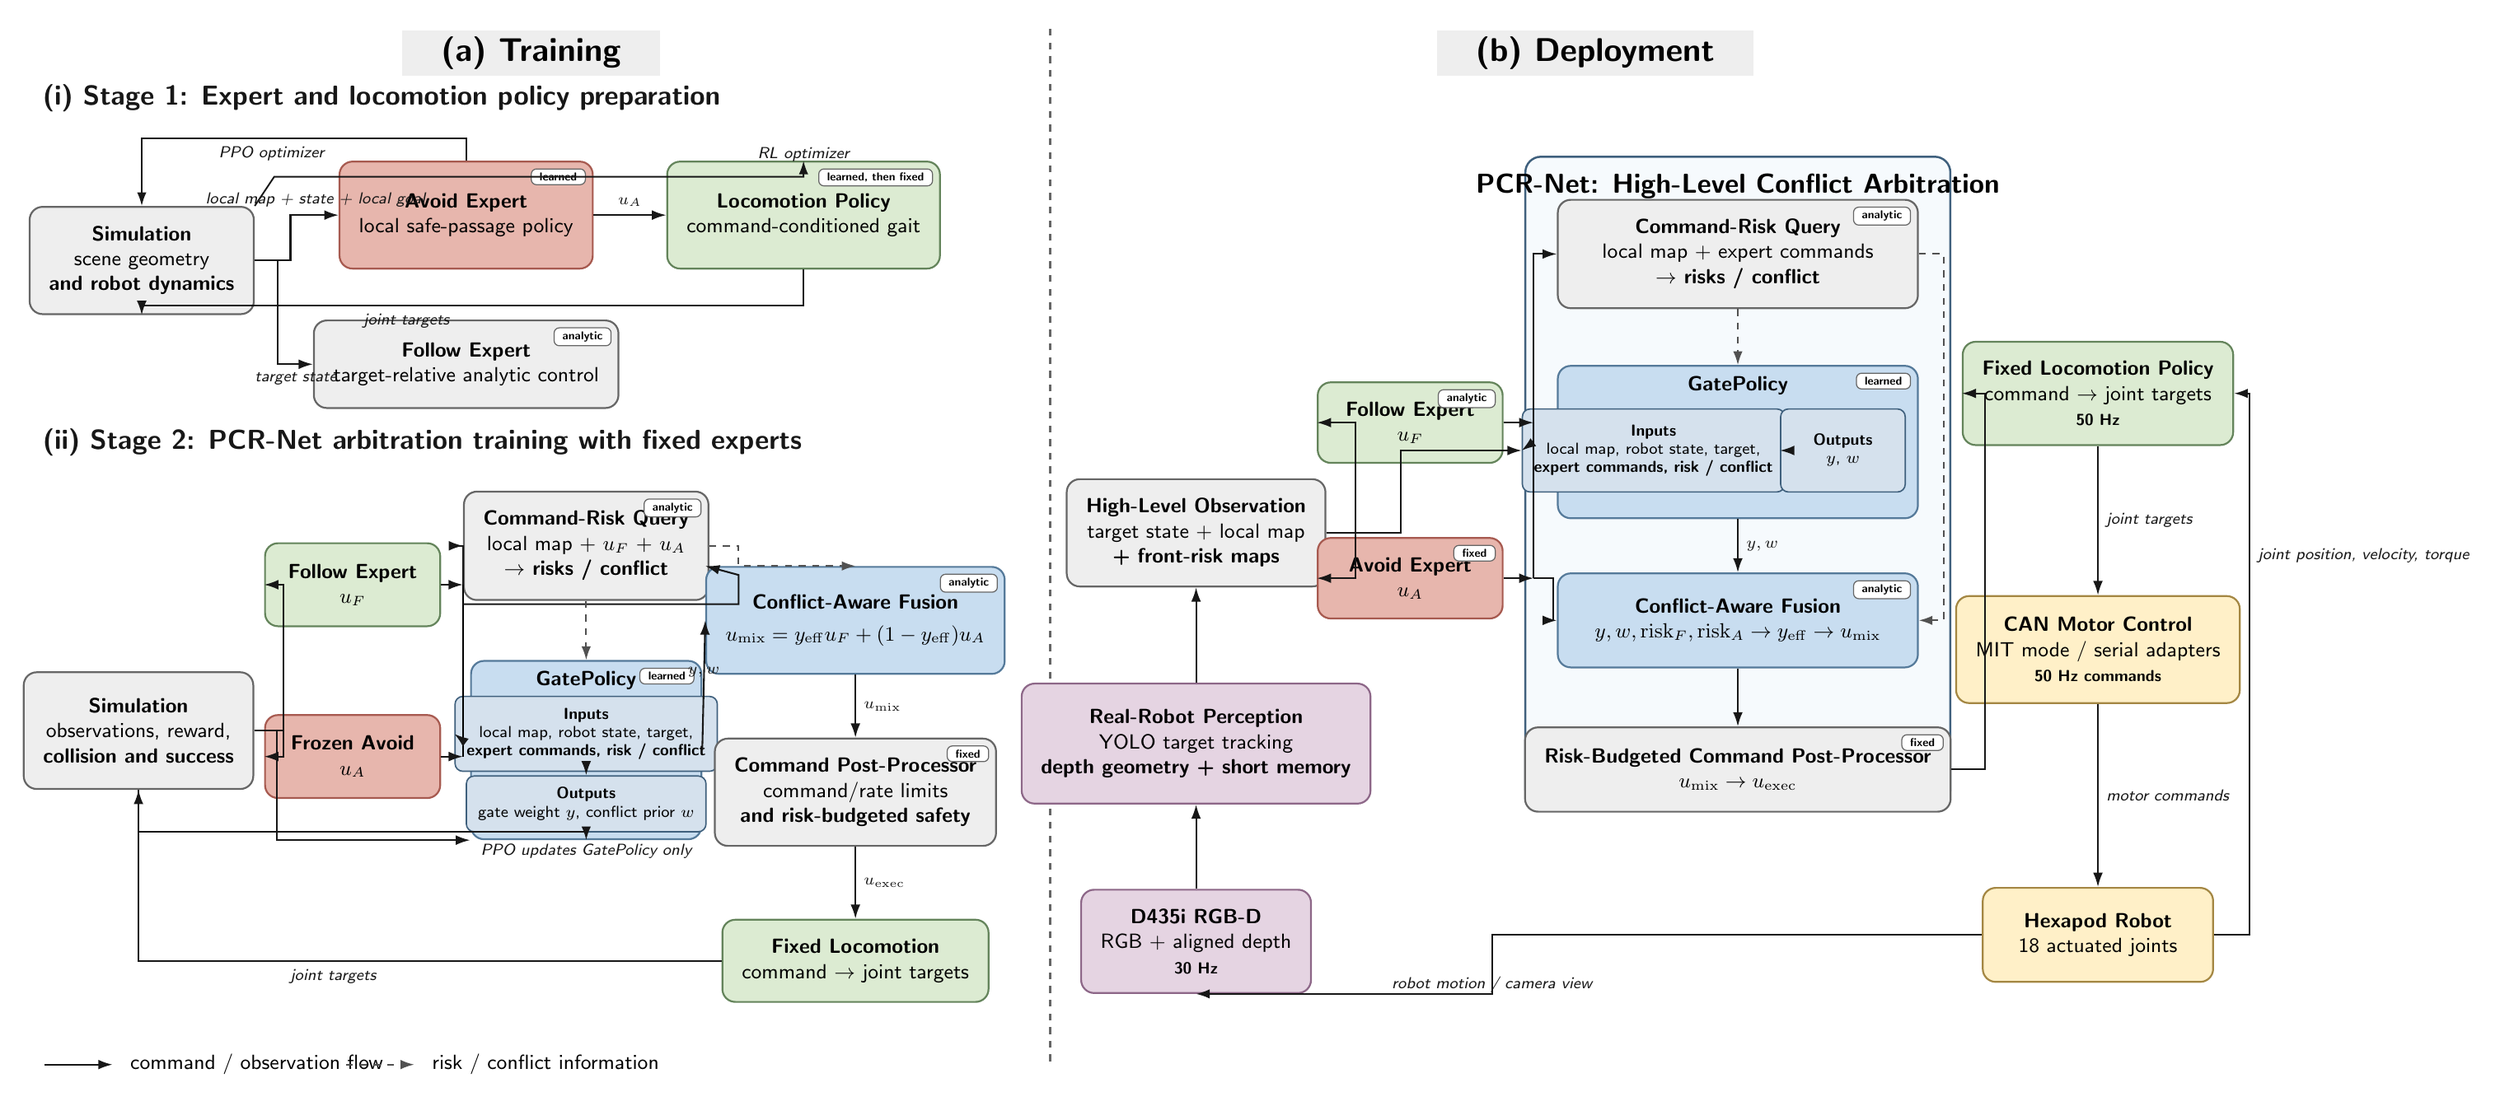
\begin{tikzpicture}[x=1cm,y=1cm]
  \node[panel] at (8.0,15.75) {(a) Training};
  \node[panel] at (24.4,15.75) {(b) Deployment};
  \draw[dashed, line width=0.9pt, graydraw] (16.0,0.2) -- (16.0,16.2);

  % ==========================================================================
  % (a) TRAINING
  % ==========================================================================
  \node[stage] at (0.35,15.05) {(i) Stage 1: Expert and locomotion policy preparation};

  \node[analytic, minimum width=3.25cm, minimum height=1.65cm] (sim1) at (2.0,12.55)
    {Simulation\\\normalfont scene geometry\\and robot dynamics};
  \node[learned, minimum width=3.35cm, minimum height=1.65cm] (avoid1) at (7.0,13.25)
    {Avoid Expert\\\normalfont local safe-passage policy};
  \node[fixed, minimum width=3.35cm, minimum height=1.65cm] (loco1) at (12.20,13.25)
    {Locomotion Policy\\\normalfont command-conditioned gait};
  \node[analytic, minimum width=3.35cm, minimum height=1.35cm] (follow1) at (7.0,10.95)
    {Follow Expert\\\normalfont target-relative analytic control};

  \node[tag, anchor=north east] at ($(avoid1.north east)+(-0.12,-0.12)$) {learned};
  \node[tag, anchor=north east] at ($(loco1.north east)+(-0.12,-0.12)$) {learned, then fixed};
  \node[tag, anchor=north east] at ($(follow1.north east)+(-0.12,-0.12)$) {analytic};

  \draw[flow] (sim1.east) -- ++(0.55,0) |- node[smalllabel,pos=0.76,above]
    {local map + state + local goal} (avoid1.west);
  \draw[feedback] (avoid1.north) -- ++(0,0.35) -| node[smalllabel,pos=0.30,below]
    {PPO optimizer} (sim1.north);
  \draw[flow] (sim1.east) -- ++(0.35,0) |- node[smalllabel,pos=0.76,below]
    {target state} (follow1.west);
  \draw[flow] (avoid1.east) -- node[smalllabel,above] {$u_A$} (loco1.west);
  \draw[flow] (loco1.south) -- ++(0,-0.55) -| node[smalllabel,pos=0.30,below]
    {joint targets} (sim1.south);
  \draw[feedback] (sim1.north east) -- ++(0.30,0.45) -| node[smalllabel,pos=0.72,above]
    {RL optimizer} (loco1.north);

  \node[stage] at (0.35,9.75) {(ii) Stage 2: PCR-Net arbitration training with fixed experts};

  \node[analytic, minimum width=3.20cm, minimum height=1.80cm] (sim2) at (1.95,5.30)
    {Simulation\\\normalfont observations, reward,\\collision and success};
  \node[fixed, minimum width=2.70cm, minimum height=1.28cm] (follow2) at (5.25,7.55)
    {Follow Expert\\\normalfont $u_F$};
  \node[learned, minimum width=2.70cm, minimum height=1.28cm] (avoid2) at (5.25,4.90)
    {Frozen Avoid\\\normalfont $u_A$};

  \node[analytic, minimum width=3.30cm, minimum height=1.55cm] (risk2) at (8.85,8.15)
    {Command-Risk Query\\\normalfont local map + $u_F$ + $u_A$\\$\rightarrow$ risks / conflict};
  \node[tag, anchor=north east] at ($(risk2.north east)+(-0.12,-0.12)$) {analytic};

  \node[gate, minimum width=3.55cm, minimum height=2.75cm] (gate2) at (8.85,5.00) {};
  \node[font=\bfseries\small] at ($(gate2.north)+(0,-0.32)$) {GatePolicy};
  \node[subblock, minimum width=2.95cm, minimum height=1.05cm] (gate2in) at ($(gate2.center)+(0,0.25)$)
    {Inputs\\\normalfont local map, robot state, target,\\expert commands, risk / conflict};
  \node[subblock, minimum width=2.95cm, minimum height=0.76cm] (gate2out) at ($(gate2.center)+(0,-0.83)$)
    {Outputs\\\normalfont gate weight $y$, conflict prior $w$};
  \draw[flow] (gate2in.south) -- (gate2out.north);
  \node[tag, anchor=north east] at ($(gate2.north east)+(-0.12,-0.12)$) {learned};

  \node[gate, minimum width=3.60cm, minimum height=1.65cm] (fusion2) at (13.00,7.00)
    {Conflict-Aware Fusion\\[1mm]
     \normalfont $\displaystyle
     u_{\mathrm{mix}}=y_{\mathrm{eff}}u_F+
     (1-y_{\mathrm{eff}})u_A$};
  \node[tag, anchor=north east] at ($(fusion2.north east)+(-0.12,-0.12)$) {analytic};

  \node[analytic, minimum width=3.60cm, minimum height=1.45cm] (post2) at (13.00,4.35)
    {Command Post-Processor\\\normalfont command/rate limits\\and risk-budgeted safety};
  \node[tag, anchor=north east] at ($(post2.north east)+(-0.12,-0.12)$) {fixed};

  \node[fixed, minimum width=3.10cm, minimum height=1.25cm] (low2) at (13.00,1.75)
    {Fixed Locomotion\\\normalfont command $\rightarrow$ joint targets};

  \draw[flow] (sim2.east) -- ++(0.45,0) |- (follow2.west);
  \draw[flow] (sim2.east) -- ++(0.45,0) |- (avoid2.west);
  % Shared expert-command bus, branched to risk query, gate, and fusion.
  \draw[flow] (follow2.east) -- (6.95,7.55);
  \draw[flow] (avoid2.east) -- (6.95,4.90);
  \draw[line width=0.75pt] (6.95,4.90) -- (6.95,7.55);
  \draw[flow] (6.95,7.55) |- (risk2.west);
  \draw[flow] (6.95,5.15) -- (gate2in.west);
  \draw[flow] (6.95,7.25) -- (11.20,7.25) -- (11.20,7.70) -- (fusion2.north west);
  \draw[flow] (sim2.east) -- ++(0.35,0) |- (gate2.south west);
  \draw[informative] (risk2.south) -- (gate2.north);
  \draw[flow] (gate2.east) -- node[smalllabel,above] {$y,w$} (fusion2.west);
  \draw[informative] (risk2.east) -- ++(0.45,0) |- (fusion2.north);
  \draw[flow] (fusion2.south) -- node[smalllabel,right] {$u_{\mathrm{mix}}$} (post2.north);
  \draw[flow] (post2.south) -- node[smalllabel,right] {$u_{\mathrm{exec}}$} (low2.north);
  \draw[flow] (low2.west) -- ++(-0.65,0) -| node[smalllabel,pos=0.32,below]
    {joint targets} (sim2.south);
  \draw[feedback] (sim2.south) -- ++(0,-0.65) -| node[smalllabel,pos=0.72,below]
    {PPO updates GatePolicy only} (gate2.south);

  % ==========================================================================
  % (b) DEPLOYMENT
  % ==========================================================================
  \node[perception, minimum width=3.15cm, minimum height=1.40cm] (camera) at (18.25,2.05)
    {D435i RGB-D\\\normalfont RGB + aligned depth\\{\scriptsize 30 Hz}};
  \node[perception, minimum width=3.90cm, minimum height=1.85cm] (percept) at (18.25,5.10)
    {Real-Robot Perception\\\normalfont YOLO target tracking\\depth geometry + short memory};
  \node[analytic, minimum width=3.70cm, minimum height=1.55cm] (obs) at (18.25,8.35)
    {High-Level Observation\\\normalfont target state + local map\\+ front-risk maps};

  \draw[flow] (camera.north) -- (percept.south);
  \draw[flow] (percept.north) -- (obs.south);

  \node[fixed, minimum width=2.85cm, minimum height=1.22cm] (followd) at (21.55,10.05)
    {Follow Expert\\\normalfont $u_F$};
  \node[learned, minimum width=2.85cm, minimum height=1.22cm] (avoidd) at (21.55,7.65)
    {Avoid Expert\\\normalfont $u_A$};
  \node[tag, anchor=north east] at ($(followd.north east)+(-0.12,-0.12)$) {analytic};
  \node[tag, anchor=north east] at ($(avoidd.north east)+(-0.12,-0.12)$) {fixed};

  \node[draw=navydraw, rounded corners=2.4mm, line width=0.9pt,
        minimum width=6.55cm, minimum height=10.00cm,
        fill=bluefill!16] (pcrbox) at (26.60,9.15) {};
  \node[font=\bfseries\large, anchor=north] at ($(pcrbox.north)+(0,-0.16)$)
    {PCR-Net: High-Level Conflict Arbitration};

  \node[analytic, minimum width=5.55cm, minimum height=1.35cm] (riskd) at (26.60,12.65)
    {Command-Risk Query\\\normalfont local map + expert commands\\$\rightarrow$ risks / conflict};
  \node[tag, anchor=north east] at ($(riskd.north east)+(-0.12,-0.12)$) {analytic};

  \node[gate, minimum width=5.55cm, minimum height=2.35cm] (gated) at (26.60,9.75) {};
  \node[font=\bfseries\small] at ($(gated.north)+(0,-0.32)$) {GatePolicy};
  \node[subblock, minimum width=2.72cm, minimum height=1.28cm] (gatedin) at ($(gated.center)+(-1.30,-0.13)$)
    {Inputs\\\normalfont local map, robot state, target,\\expert commands, risk / conflict};
  \node[subblock, minimum width=1.92cm, minimum height=1.28cm] (gatedout) at ($(gated.center)+(1.62,-0.13)$)
    {Outputs\\\normalfont $y$, $w$};
  \draw[flow] (gatedin.east) -- (gatedout.west);
  \node[tag, anchor=north east] at ($(gated.north east)+(-0.12,-0.12)$) {learned};

  \node[gate, minimum width=5.55cm, minimum height=1.45cm] (fusiond) at (26.60,7.00)
    {Conflict-Aware Fusion\\\normalfont
      $y,w,\mathrm{risk}_F,\mathrm{risk}_A
      \rightarrow y_{\mathrm{eff}}\rightarrow u_{\mathrm{mix}}$};
  \node[tag, anchor=north east] at ($(fusiond.north east)+(-0.12,-0.12)$) {analytic};

  \node[analytic, minimum width=5.55cm, minimum height=1.30cm] (postd) at (26.60,4.70)
    {Risk-Budgeted Command Post-Processor\\\normalfont
      $u_{\mathrm{mix}}\rightarrow u_{\mathrm{exec}}$};
  \node[tag, anchor=north east] at ($(postd.north east)+(-0.12,-0.12)$) {fixed};

  \draw[flow] (obs.east) -- ++(0.45,0) |- (followd.west);
  \draw[flow] (obs.east) -- ++(0.45,0) |- (avoidd.west);
  % Shared expert-command bus.
  \draw[flow] (followd.east) -- (23.45,10.05);
  \draw[flow] (avoidd.east) -- (23.45,7.65);
  \draw[line width=0.75pt] (23.45,7.65) -- (23.45,10.05);
  \draw[flow] (23.45,10.05) |- (riskd.west);
  \draw[flow] (23.45,9.75) -- (gatedin.west);
  \draw[flow] (23.45,7.65) -- (23.75,7.65) |- (fusiond.west);
  \draw[flow] (obs.east) -- ++(1.15,0) |- (gatedin.west);
  \draw[informative] (riskd.south) -- (gated.north);
  \draw[flow] (gated.south) -- node[smalllabel,right] {$y,w$} (fusiond.north);
  \draw[informative] (riskd.east) -- ++(0.38,0) |- (fusiond.east);
  \draw[flow] (fusiond.south) -- (postd.north);

  \node[fixed, minimum width=3.30cm, minimum height=1.55cm] (lowd) at (32.15,10.50)
    {Fixed Locomotion Policy\\\normalfont command $\rightarrow$ joint targets\\{\scriptsize 50 Hz}};
  \node[control, minimum width=3.30cm, minimum height=1.65cm] (cand) at (32.15,6.55)
    {CAN Motor Control\\\normalfont MIT mode / serial adapters\\{\scriptsize 50 Hz commands}};
  \node[control, minimum width=3.55cm, minimum height=1.45cm] (robot) at (32.15,2.15)
    {Hexapod Robot\\\normalfont 18 actuated joints};

  \draw[flow] (postd.east) -- ++(0.52,0) |- (lowd.west);
  \draw[flow] (lowd.south) -- node[smalllabel,right] {joint targets} (cand.north);
  \draw[flow] (cand.south) -- node[smalllabel,right] {motor commands} (robot.north);
  \draw[feedback] (robot.east) -- ++(0.55,0) |- node[smalllabel,pos=0.35,right]
    {joint position, velocity, torque} (lowd.east);
  \draw[feedback] (robot.west) -- ++(-7.55,0) |- node[smalllabel,pos=0.28,below]
    {robot motion / camera view} (camera.south);

  % Legend.
  \draw[flow] (0.50,0.15) -- (1.55,0.15);
  \node[font=\small,anchor=west] at (1.70,0.15) {command / observation flow};
  \draw[informative] (5.15,0.15) -- (6.20,0.15);
  \node[font=\small,anchor=west] at (6.35,0.15) {risk / conflict information};
\end{tikzpicture}
\end{document}
